As illustrated by Figure {equivalent_circuit}, the rectifier consists of a single diode as the source of nonlinearity and a low-pass filter to store energy. Assume lossless, the equivalent circuit includes a voltage source ${v_{\text{s}}}(t)$ connected to a series antenna impedance ${Z_{{\text{ant}}}} = {R_{{\text{ant}}}} + j{X_{{\text{ant}}}}$ followed by a combined impedance of the rectifier and the matching network ${Z_{{\text{in}}}} = {R_{{\text{in}}}} + j{X_{{\text{in}}}}$, as shown in Figure {equivalent_circuit}. When perfect matched (${R_{{\text{in}}}} = {R_{{\text{ant}}}},{X_{{\text{in}}}} =  - {X_{{\text{ant}}}}$), the voltage across the rectifier equals ${v_{{\text{in}}}}(t) = {v_{\text{s}}}(t)/2 = {y_{{\text{rf}}}}(t)\sqrt {{R_{{\text{in}}}}} $ and the input power to the rectifier writes $P_{{\text{rf}}}^r = \mathbb{E}\left[ {{y_{{\text{rf}}}}{{(t)}^2}} \right] = \mathbb{E}\left[ {{v_{{\text{in}}}}{{(t)}^2}} \right]/{R_{{\text{in}}}}$. It is assumed that the noise is too small to be harvested.

\begin{figure}
  \centering
    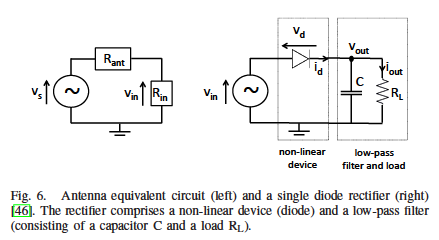
\includegraphics[width=0.5\textwidth]{Rectenna equivalent circuit and a single diode rectifier}
  \caption{Rectenna equivalent circuit (left) and a single diode rectifier (right) \cite{Clerckx2018a}}
  \label{fig:rectenna_circuit}
\end{figure}